\chapter{Warstwa pośrednia w zastosowaniu }
\label{cha:example}

Najlepszym sposobem weryfikacji każdego rozwiązania jest jego konfrontacja z rzeczywistością, przez znalezienie realnych przykładów jego użycia. Nie inaczej jest w~przypadku proponowanego w niniejszej pracy rozwiązania. 

Pomysłem na przykład jest w tym przypadku proces sprzątania pokoju hotelowego. Celem przykładu jest zademonstrowanie działania warstwy pośredniej do komunikacji procesu biznesowego z aplikacjami mobilnymi, ale również pokazania sposobu integracji takiego rozwiązania z gotowymi systemami zewnętrznymi. 

%---------------------------------------------------------------------------

\section{Przedstawienie koncepcji}
\label{sec:concept}

Prezentacja przykładu zostanie rozpoczęta od przedstawienia koncepcji rozwiązania w postaci diagramów zaprojektowany za pomocą BPMN 2.0. Przedstawione zostaną dwa diagramy z których pierwszy jest sytuacją w której rozpoczyna się właściwy proces sprzątania hotelu. 

\begin{figure}[h]
\centerline{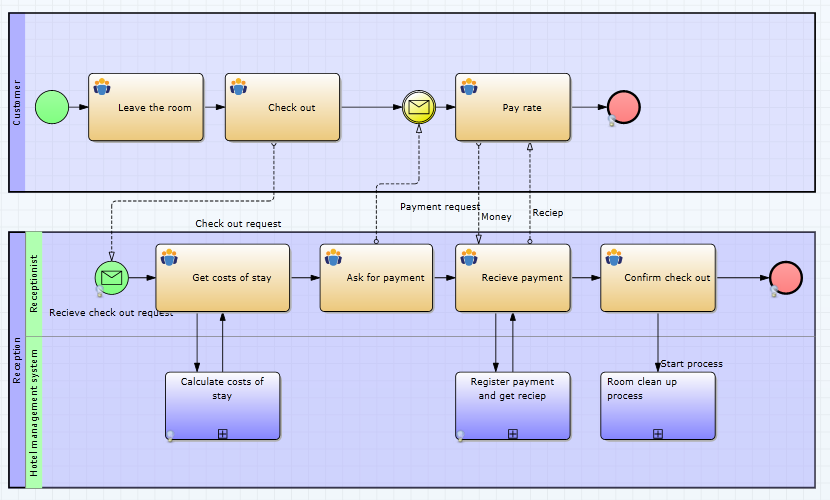
\includegraphics[scale=0.5]{hotelCheckOutProcess}}
\caption{Diagram BPMN procesu wymeldowania klienta z pokoju hotelowego.}
\label{fig:hotelCheckOutProcess}
\end{figure}

Na rysunku ~\ref{fig:hotelCheckOutProcess}, przedstawiono proces wymeldowania gościa hotelowego z pokoju po zakończonym pobycie. Klient hotelu po opuszczeniu pokoju udaje się do recepcji w celu oddania kluczy i uregulowania płatności. W~recepcji przebywa recepcjonista, który odpowiedzialny jest za kontakt z klientem, po otrzymaniu kluczy prosi klienta o zapłatę kosztów pobytu. Po dokonaniu płatności klient hotelowy opuszcza hotel, a~recepcjonista oznacza pokój hotelowy jako gotowy do posprzątania, rozpoczynając w~ten sposób właściwy proces. 

\begin{figure}[h]
\centerline{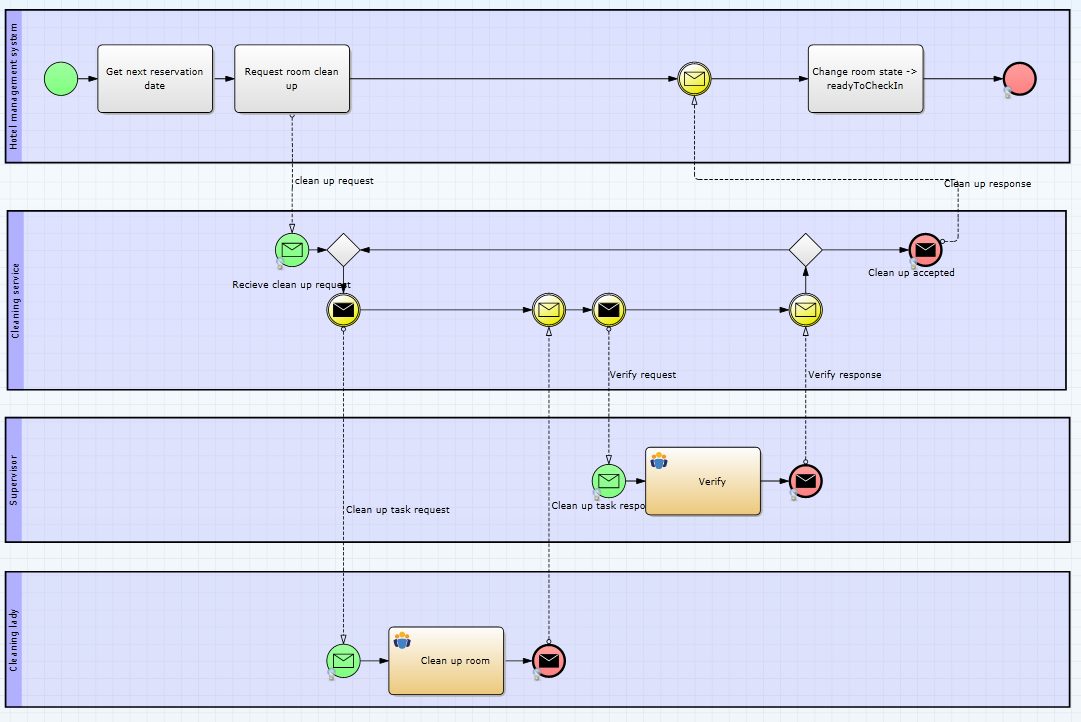
\includegraphics[scale=0.45]{roomCleanUpProcess}}
\caption{Diagram BPMN procesu sprzątania pokoju hotelowego.}
\label{fig:roomCleanUpProcess}
\end{figure}

Rysunek~\ref{fig:roomCleanUpProcess} przedstawia właściwy proces sprzątania pokoju hotelowego, widać na nim cztery rodzaje aktorów, każdy z nich oznaczony własną linią. Pierwszym z aktorów jest system zarządzania hotelem, jest to miejsce w którym recepcjonista oznacza pokój do posprzątania. System zarządzania hotelem jest miejscem w którym rozpoczyna się proces. Odpowiedzialny jest on za zebranie danych koniecznych do przeprowadzenia sprzątania a następnie przekazanie tych danych do kolejnego aktora, którym jest Serwis Sprzątający. A przypadku realizacji przykładu za pomocą opisanych w niniejszej pracy magisterskiej technologii, aktora tego można utożsamić z procesem BPEL wraz z warstwą pośrednią. Ostani aktor - serwis sprzątający odpowiedzialny jest za przeprowadzenie procesu sprzątania. Proces ten odbywa się przez wysłanie żądania do sprzątaczki (aplikacja mobilna), by po potwierdzeniu posprzątania pokoju wysłać żądanie do nadzorcy (również aplikacja mobilna) który będzie odpowiedzialny za weryfikacje sprzątania.  W przypadku braku akceptacji sprzątania przez nadzorcę pokój będzie musiał być kolejny raz posprzątany. W momencie zatwierdzenia sprzątania, rezultat trafi ponownie do Systemu Zarządzania Hotelem, aby recepcjonista mógł zameldować kolejnych gości. 

Na podstawie opisanego powyżej przykładu wyłonić można następujące systemy, których implementacja zostanie dokładniej opisana w dalszej części pracy.

\begin{itemize}
\item System Zarządzania Hotelem -- Dla celów przykładu, System Zarządzania Hotelem będzie prostą aplikacją internetową odpowiedzialną za udostępnienie formularza dla recepcjonisty oraz wyświetlenie listy rezultatów wykonania procesu.   
\item Proces BPEL -- Będzie to proces zawierający kompletną logikę biznesową odpowiedzialną za przeprowadzenie i weryfikacje sprzątania pokoju hotelowego. Proces ten będzie komunikował się zarówno z warstwą pośrednią jak i z Systemem Zarządzania Hotelem. 
\item Warstwa pośrednia --  Aplikacja internetowa odpowiedzialna za obsługę komunikacji procesu biznesowego z aplikacjami mobilnymi. 
\item Aplikacja mobilna -- aplikacja przeznaczona zarówno dla sprzątaczek jak i dla nadzorców. Udostępniać będzie bardzo prosty interfejs użytkownika służący do wyświetlenia listy zadań oraz do ich przypisywania i rozwiązywania. 
\end{itemize}


%---------------------------------------------------------------------------

\section{System Zarządzania Hotelem }
\label{sec:hotelManagementSystem}

Zadaniem tej aplikacji jest udostępnienie części funkcjonalność Systemu Zarządzania Hotelem przeznaczonej do oznaczania pokoju hotelowego jako wymagającego posprzątania. Aplikacja udostępniać będzie formularz w którym recepcjonista będzie mógł zgłosić pokój do posprzątania. Formularz będzie gromadził taki dane jak numer pokoju, numer piętra oraz kategorię do której należy pokój. Po zatwierdzeniu formularza  dane z niego pochodzące trafią do procesu biznesowego oraz do bazy danych w celu monitorowania postępu procesu. Kiedy proces zakończy swoje działania aplikacja odbierze za pomocą odpowiedniej usługi sieciowej jego rezultat. Odebranie rezultatu skutkować będzie zmianą statusu pokoju. Aplikacja udostępniać będzie również listę pokoi wraz z ich statusami w postaci strony www. 

\subsection{Wybrane technologie}
Aplikacja zostanie zrealizowana przy wykorzystaniu technologii:

\begin{itemize}
\item język programowania Java
\item Spring MVC
\item  Bootstrap Framework -- jest to zbiór  klas css oraz biblioteka stworzona w języku JavaScript, służący do tworzenia interfejsu użytkownika przy pomocy zaawansowanych kontrolek html.
\item Maven
\item Spring Web Services
\item Spring Data oraz Hibernate - jeden z najbardziej popularnych narzędzi ORM, przeznaczonych na platformę Java. 
\item H2 in memory - baza danych której cykl życia jest równoznaczny z cyklem życia aplikacji. Jest ona tworzona podczas uruchamiana aplikacji, dane znajdujące w się w niej są przechowywane w pamięci podręcznej. Bazy tego typu wykorzystywane są przede wszystkim do implementacji testów jednostkowych. Zdecydowanym plusem skorzystania z tego rodzaju bazy danych jest brak konieczności instalacji dodatkowych narzędzi co w przypadku niniejszego przykładu jest dużym udogodnieniem. 
\end{itemize}

\subsection{Implementacja}

\begin{figure}[h]
\centerline{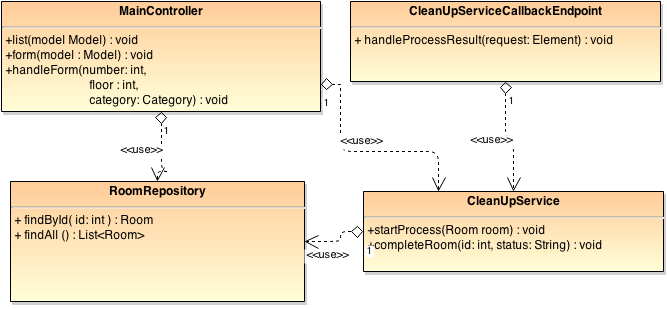
\includegraphics[scale=0.6]{hotelManagementSystemClasses}}
\caption{Diagram klas systemu zarządzania hotelem.}
\label{fig:hotelManagementSystemClasses}
\end{figure}


Na rysunku~\ref{fig:hotelManagementSystemClasses} został przedstawiony diagram klas Systemu Zarządzania Hotelem. Znajdują się na nim jedynie najbardziej istotne klasy z punku widzenia tej implementacji. Klasa \textit{MainController} jest odpowiedzialna za udostępnienie interfejsu użytkownika oraz za obsługę żądań z niego pochodzących. Udostępnia ona trzy metody: 


\begin{itemize}
\item \textit{list} -- metoda za pomocą RomRepository pobiera z bazy danych wszystkie pokoje, które zostały zgłoszone do posprzątania. Pobrana lista jest  następnie umieszczana w dynamicznej stronie www za pomocą technologii JSP. 
\item \textit{form} -- metoda odpowiedzialna za wyświetlenie formularza w postaci html dla użytkownika. 
\item \textit{hadleForm} -- metoda ta jest uruchamiana w przypadku zatwierdzenia danych wprowadzonych do formularza przez użytkownika. Metoda dodaje nowy pokój do bazy danych oraz uruchamia proces biznesowy z wykorzystaniem klasy \textit{CleanUpService}. 
\end{itemize}

Druga bardzo ważną klasą jest \textit{CleanUpServiceCallbackEndpoint}, jest to klasa stworzona z wykorzystaniem technologii Spring Web Services. Klasa ta obsługuje zdefiniowaną w konfiguracji usługę sieciową. Usługa służy do odbierania rezultatów wykonania procesu biznesowego. Jej rolą jest przeczytania komunikatu przysłanego przez proces biznesowy by następnie zmienić status sprzątanego pokoju za pomocą klasy \textit{CleanUpService}. 

\subsection{Uruchomienie}

Aplikacja jest kompilowana do postaci pliku o rozszerzeniu war. Pliki tego typu mogą być uruchamiana na dowolnym serwerze aplikacyjnym Java, np. Tomcat. Aplikacja powinna zostać uruchomiona na porcie 8181, ponieważ pozostałe aplikacje będą od niej tego wymagały. Np. proces biznesowy swój rezultat będzie wysyłał właśnie do lokalnej maszyny na ten port. 

%---------------------------------------------------------------------------

\section{Proces BPEL }
\label{sec:exampleBPEL}

Proces BPEL jest odpowiedzialny za obsługę logiki biznesowej związanej z przeprowadzeniem procesu sprzątania. Proces służy w pewnym sensie jako narzędzie integracyjne aplikację internetową jaką jest System Zarządzania Hotelem z aplikacjami mobilnymi. 

Przebieg działania procesu rozpoczyna się w Systemie Zarządzania Hotelem, który uruchamia usługę sieciową udostępnianą jako punkt dostępowy procesu. Proces po otrzymaniu żądania z systemu zewnętrznego tworzy nowe zadanie przeznaczone dla osoby sprzątającej pokój by następnie przejść w tryb oczekiwania na jego rezultat. Gdy pokój zostanie posprzątany, proces tworzy kolejne zadanie tym razem przeznaczone dla nadzorcy i ponownie przechodzi w tryb oczekiwania na jego rezultat. Gdy nadzorca zakończy swoje zadanie proces sprawdzi jego rezultat, jeśli sprzątanie pokoju zostało zaakceptowane proces zakończy swoje działanie poprzez wysłanie rezultatu do Systemu Zarządzania Hotelem. Gdy sprzątanie pokoju nie zostanie zaakceptowane proces będzie tworzył  kolejne zadania dla osoby sprzątającej do momentu zatwierdzenia przez nadzorcę. 

\subsection{Implementacja}

\begin{figure}[h]
\centerline{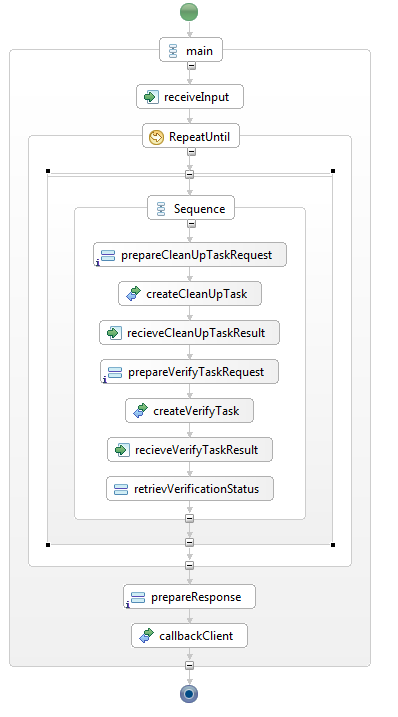
\includegraphics[scale=0.6]{bpelProcess}}
\caption{Wizualizacja procesu BPEL w postaci graficznej za pomocą wtyczki do Eclipsa.}
\label{fig:bpelProcess}
\end{figure}

Do implementacji procesu BPEL została wykorzystana wtyczka do zintegrowanego środowiska programistycznego Eclipse. Wtyczka ta udostępnia narzędzia do modelowania procesów BPEL w sposób graficzny. Na rysunku~\ref{fig:bpelProcess} został przedstawiony zrzut ekranu przedstawiający implementację niniejszego procesu biznesowego. Na rysunku widać doskonale kolejność wywoływania poszczególnych aktywności procesu BPEL, nie widać natomiast zastosowania mechanizmu korelacji oraz zakresu. 

\subsubsection{Korelacja}

Mechanizmem na który w szczególności należy zwrócić uwagę podczas opisu procesu biznesowego jest mechanizm korelacji. Mechanizm ten służy do powiązania dwóch lub więcej operacji wewnątrz jednej instancji procesu. W przypadku niniejszego przykładu proces korelacji wykorzystywany jest do powiązywania operacji stworzenie zadania z operacją odebrania rezultatu zadania. Zazwyczaj środowisko uruchomieniowe posiada więcej niż jedną instancje procesu, w momencie gdy zostaje odebrany rezultat zadania np. sprzątania środowisko powinno w jakiś sposób zidentyfikować instancję procesu do której zaadresowany jest ten rezultat. 

Mechanizm korelacji realizowany jest za pomocą tak zwanych zbiorów korelacji. Zbiór korelacji nie jest niczym innym jak zbiorem zmiennych. Zmienne te inicjalizowane są przy pierwszym użyciu dowolną wartością, podczas kolejnego użycia służą do odszukania instancji procesu o zadanej wartości. 

W niniejszym procesie istnieją dwa zbiory korelacji, zdefiniowane wewnątrz ciała pętli: 

\begin{lstlisting}[caption=Definicja zbiorów korelacji.,numbers=left]
<bpel:correlationSets>
	<bpel:correlationSet name="cleanUpTask" 
			properties="tns:taskUUID"/>
	<bpel:correlationSet name="verifyTask" 
			properties="tns:verifyTaskUUID"/>
</bpel:correlationSets> 


\end{lstlisting}

Zbiory te wykorzystywane są do powiązania operacji stworzenia i odbioru rezultatu zadania sprzątanie i weryfikacja. 

\begin{lstlisting}[caption=Wykorzystanie zbiorów korelacji w aktywności invoke.,numbers=left]
<bpel:receive name="recieveCleanUpTaskResult" partnerLink="client" 
	operation="cleanUpTaskCallback" portType="tns:cleanUpProcess" 
	variable="clientRequest">
            <bpel:correlations>
                <bpel:correlation set="cleanUpTask" initiate="no">
	     </bpel:correlation>    
            </bpel:correlations>
        
</bpel:receive>
\end{lstlisting}

Operacja invoke odpowiedzialna za stworzenie zadania inicjalizuje zbiór korelacji odebraną z warstwy pośredniej wartością unikalnego identyfikatora zadania.

\begin{lstlisting}[caption=Wykorzystanie zbiorów korelacji w aktywności receive.,numbers=left]
<bpel:receive name="recieveCleanUpTaskResult" partnerLink="client" 
		operation="cleanUpTaskCallback"
	          portType="tns:cleanUpProcess" variable="clientRequest">
            <bpel:correlations>
                	<bpel:correlation set="cleanUpTask" initiate="no">
		</bpel:correlation>    
            </bpel:correlations>
</bpel:receive>

\end{lstlisting}

 Operacja recieve następnie na podstawie tego samego unikalnego identyfikatora odnajduje odpowiednią instancje by kontynuować jej działanie. 

\subsubsection{Zakres }
Bezpośrednio powiązany z mechanizmem korelacji jest mechanizm zakresów (ang. scope). Służy on do odizolowania dwóch lub więcej operacji wewnątrz procesu. Izolacja ta może zostać wykorzystana np. do odpowiedniego zarządzania sytuacjami wyjątkowymi. W przypadku niniejszego procesu mechanizm zakresu został zastosowany do odizolowania kolejnych wywołań pętli w celu uzyskania efektu ponownej inicjalizacji zbiorów korelacji w każdym przebiegu pętli. W przypadku nie zastosowania mechanizmy zakresu, podczas pierwszego wywołania przebiegu pętli zbiór korelacji zostałby zainicjalizowany identyfikatorem pierwszego zadania. W przypadku kolejnych wywołań pętli metoda recieve oczekiwała by na identyfikator pierwszego zadania mimo, że zostało ono już rozwiązane a kolejny przebieg pętli stworzył następne zadanie. 

Mechanizm zakresu stosuje się obejmując izolowane elementy w drzewie xml elementem \textit{scope}.

\subsection{Uruchomienie}
 Proces BPEL został stworzony zgodnie ze specyfikacją BPEL, może być zatem wdrożony na dowolne środowisko uruchomieniowe dla procesów biznesowych. W przykładzie zastosowano środowisko Apache ODE. 

Apache ODE jest również aplikacją internetową napisaną w języku Java i może być uruchomiony z~wykorzystaniem dowolnego serwera aplikacyjnego. Ważne jest aby silnik Apache ODE został uruchomiony z wykorzystaniem portu 8080. System Zarządzania Hotelem będzie próbował uruchomić proces na lokalnej maszynie pod tym właśnie portem.  


%---------------------------------------------------------------------------


\section{Warstwa pośrednia }
\label{sec:exampleMiddleware}

Najbardziej istotną częścią przykładu z punktu widzenia niniejszej pracy magisterskiej jest warstwa pośrednia. Jest ona odpowiedzialna za odbiór  żądań od procesu biznesowego i przekazanie ich do aplikacji mobilnych. Warstwa pośrednia udostępnia w tym celu dwie usługi sieciowe. Jedną do utworzenia zadania - sprzątanie pokoju i drugą do utworzenia zadania - weryfikacja sprzątania. Żądania odbierane przez usługi sieciowe zapisywane są następnie w dokumentowej bazie danych i oczekują na realizacje przez użytkowników mobilnych. Aplikacje mobilne komunikują się warstwą pośrednią za pomocą REST API. Są w stanie w ten sposób zautoryzować się, pobrać listę zadań i rozwiązywać je. Zadania po rozwiązaniu odsyłane są do procesów biznesowego z wykorzystaniem odpowiednich usług sieciowych. 

\subsection{Wybrane technologie}
Warstwa pośrednia z racji tego, że wykorzystuje przedstawioną w niniejszej pracy magisterskiej bibliotekę, została zrealizowana w technologii Spring i korzysta z bazy danych Mongo DB.

\subsection{Implementacja}

Jak wspomniano wcześniej warstwa pośrednia wykorzystuje opisaną w niniejszej pracy magisterskiej bibliotekę stworzoną do tego celu. Opis implementacji zaczniemy od dwóch najważniejszych plików konfiguracyjnych tej biblioteki. Pierwszym z nich jest plik bpel4mobile.properties znajdujący się w katalogu resources. W pliku tym znajdują się dane do komunikacji z bazą danych MondoDB, oraz ścieżka do drugiego pliku konfiguracyjnego - humanInteractions.xml. Plik xml jest najważniejszym plikiem konfiguracyjnym z punktu widzenia stworzonej biblioteki, zawiera od definicje zadań, grup użytkowników i przypisania poszczególnych grup do zadań. 

\begin{lstlisting}[caption=Plik konfiguracyjny z opisem zadań warstwy pośredniej.,numbers=left]
<?xml version="1.0" encoding="UTF-8"?>
<htd:humanInteractions
	xmlns:htd="http://docs.oasis-open.org/bpel4people/ws-humantask"
	xmlns:xsi="http://www.w3.org/2001/XMLSchema-instance"
	xmlns:xsd="http://www.w3.org/2001/XMLSchema"
	xsi:schemaLocation="http://docs.oasis-open.org/ bpel4people/ws-humantask  http://docs.oasis-open.org/bpel4people/ws-humantask.xsd">

	<htd:logicalPeopleGroups>
		<htd:logicalPeopleGroup name="cleaningLadies">
			<htd:parameter name="correspondingFloor" type="xsd:int"/>
		</htd:logicalPeopleGroup>
		<htd:logicalPeopleGroup name="supervisors" />
	</htd:logicalPeopleGroups>
	<htd:tasks>
		<htd:task name="cleanUpTask">
			<htd:priority>5</htd:priority>
			<htd:peopleAssignments>
				<htd:potentialOwners>
					<htd:from  logicalPeopleGroup="cleaningLadies">
					<htd:argument  name="correspondingFloor">
						eq:request/room/floor
					</htd:argument>
					</htd:from>
				</htd:potentialOwners>
			</htd:peopleAssignments>
		</htd:task>
		<htd:task name="verifyTask">
			<htd:priority>5</htd:priority>
			<htd:peopleAssignments>
				<htd:potentialOwners>
				<htd:from logicalPeopleGroup="supervisors" />
				</htd:potentialOwners>
			</htd:peopleAssignments>
		</htd:task>
	</htd:tasks>
</htd:humanInteractions>
\end{lstlisting}

Na powyższym fragmencie kodu widoczny jest pliku konfiguracyjny niniejszego przykładu. Linijki 8-13 zawierają definicję dwóch grup użytkowników, jednej dla sprzątaczek i drugiej dla nadzorców. Sprzątaczki posiadają dodatkowy atrybut którym jest numer piętra na którym pracują. W elemencie \textit{tasks} znajdują się definicję zadań, widać na nich, że zadanie sprzątania przypisane jest do sprzątaczek pracujących na danym piętrze, natomiast weryfikację mogą przeprowadzać dowolni nadzorcy. Sposób konfiguracji zadań jest bardzo prosty, przejrzysty i elastyczny. 

Kolejną ważną częścią implementacji warstwy pośredniej jest udostępnienie usług sieciowych dla procesu biznesowego. Zadanie to zrealizowane zostaje przy pomocy modułu Spring WS. Spring WS do tworzenia usług sieciowych preferuje podejście interfejs najpierw (ang. contract first), w celu udostępnienia usług sieciowej konieczne jest zdefiniowanie pliku ze schematem komunikatów xml. Powstają w tej sposób dwa pliki dla dwóch różnych usług sieciowych. Pliki te wykorzystane zostaną do wygenerowanie odpowiednich kontraktów WSDL przez Spring WS. Po stronie kodu Java, powstają odpowiedniki opisanych komunikatów w postaci klas. Po dwie klasy na usługę sieciową do obsługi wiadomości wejściowej i rezultatu. Przykładowo dla weryfikacji sprzątania klasy będą wyglądać następująco: 

\begin{lstlisting}[caption=Klasy zawierające komunikaty wejściowe i wyjściowe usługi weryfikacji sprzątania.,numbers=left]
@XmlRootElement(name="request", namespace= XMLNamespace.VERIFY)
public class VerifyRequest {

	@XmlElement(name="deadline",
		namespace=XMLNamespace.VERIFY)
	private Date deadline;

	@XmlElement(name="cleanUpPerformer", 
		namespace=XMLNamespace.VERIFY)
	private String cleanUpPerformer;

	@XmlElement(name="room", 
		namespace=XMLNamespace.VERIFY)
	private Room room;
}

@XmlRootElement(name="result", namespace="http://bpel4mobile.com/example/hotel/schemas")
public class VerifyResponse {

	public enum Status {
		success, toRepeat
	}

	@XmlElement(name="status",  namespace="http://bpel4mobile.com/example/hotel/schemas")
	private Status status;
}
\end{lstlisting}

Spring WS oprócz przygotowania plików ze schematem xml komunikatów, wymaga zdefiniowanie servletu w plikach xml. Servlet ten wskazuje na pliki ze schematem xml oraz definiuje przestrzeń nazw i port usługi sieciowej. 

\begin{lstlisting}[caption=Servlet usługi weryfikacji sprzątania.,numbers=left]
<beans ... >
	<sws:dynamic-wsdl id="verifyService"  	portTypeName="verifyServicePort" 
		locationUri="http://localhost:8282/hotel-cleanup-mobile-middleware/ws/verifyService" 
		targetNamespace="http://bpel4mobile.com/ schemas/example/verifyService"> 
	<sws:xsd location="/WEB-INF/schema/verify-request.xsd"/> 
	</sws:dynamic-wsdl>
</beans>
\end{lstlisting}

Ostatnią rzeczą do implementacji w celu udostępnienia usługi sieciowej jest przygotowanie odpowiedniej klasy Java która będzie punktem końcowym zdefiniowanego wcześniej servletu. Klasa ta będzie uruchamiać odpowiednią instancję serwisu do obsługi zadań zdefiniowanych w warstwie pośredniej. Dalszą obsługą zadania wraz z odesłaniem odpowiedzi zajmie się przygotowana w poprzednim rozdziale biblioteka. 

\begin{lstlisting}[caption=Punkt końcowy usługi weryfikacji sprzątania.,numbers=left]
@Endpoint
public class VerifyServiceEndpoint {

	@Autowired
	@Qualifier(value="verifyTaskService")
	private TaskService tasService;

	@PayloadRoot(namespace = XMLNamespace.VERIFY,  localPart = "VerifyTaskRequest") 
	@ResponsePayload
	public Element handleHolidayRequest(@RequestPayload Element request) throws Exception {
		return tasService.handleTaskRequest(request,  VerifyRequest.class,  VerifyResponse.class);
	}
}
\end{lstlisting}

Do zakończenia implementacji warstwy pośredniej konieczne jest jeszcze dostarczenie informacji o użytkownikach systemu. Biblioteka utworzona w poprzednim rozdziale przewiduje do tego celu odpowiedni interfejs, który zostanie zaimplementowany. Na potrzeby niniejszego przykładu nie konieczne jest tworzenie adaptera do pobierania danych o użytkownikach z bazy danych czy innych systemów katalogowych, utworzymy prostą klasę dostarczającą statyczne dane. 

\begin{lstlisting}[caption=Dostawca informacji o użytkownikach. =,numbers=left]
@Service
public class UserDataProviderImpl  extends AbstractUserDataProvider {

	private Map<String, UserData> users =  new HashMap<String, UserData>();

	@PostConstructor
	public void init(){
		UserGroupData cleanUpGroupDataFloor1 = new UserGroupData();
		cleanUpGroupDataFloor1.setName("cleaningLadies");
		cleanUpGroupDataFloor1.getArguments().put("correspondingFloor", 1);

		UserGroupData cleanUpGroupDataFloor2 = new UserGroupData();
		cleanUpGroupDataFloor2.setName("cleaningLadies");
		cleanUpGroupDataFloor2.getArguments() .put("correspondingFloor", 2);

		UserGroupData supervisorGroup = new UserGroupData();
		supervisorGroup.setName("supervisors");

		UserData jadzia = new UserData();
		jadzia.setUsername("Jadzia");
		jadzia.getGroups().add(cleanUpGroupDataFloor1);
		users.put("Jadzia", jadzia);

		UserData stasia = new UserData();
		stasia.setUsername("Stasia");
		stasia.getGroups().add(cleanUpGroupDataFloor2);
		users.put("Stasia", stasia);

		UserData zdzislaw = new UserData();
		zdzislaw.setUsername("Zdzislaw");
		zdzislaw.getGroups().add(supervisorGroup);
		users.put("Zdzislaw", zdzislaw);
	}
	@Override
	public boolean authenticate(String username, 
				String password) {
		return (users.contains(username) && "password".equals(password));
	}

	@Override
	public UserData getUserData(String username, String password) {
		return users.get(username);
	}
}
\end{lstlisting}

\subsection{Uruchomienie}

Aplikacja budowana jest za pomocą narzędzia maven. Plikiem wynikowym podobnie jak w przypadku systemu zarządzania hotelem jest plik z rozszerzeniem .war, który można uruchomić na dowolnym serwerze aplikacyjnym java. Warstwa pośrednia aby współgrała z pozostałymi systemami, musi zostać uruchomiona na porcie 8282. 

%---------------------------------------------------------------------------

\section{Aplikacja mobilna}
\label{sec:exampleMobileApp}

Aplikacja mobilna jest częścią przykładu odpowiedzialną za rozwiązywanie zadań poprzez udostępnienie użytkownikom odpowiedniego interfejsu. Aplikacja komunikuje się w warstwą pośrednią za pomocą REST API w celu pobrania listy zadań, operacji na tych zadaniach i wysłania rezultatu. Aplikacja została zaimplementowana na najbardziej popularną platformę mobilną - Android. 

Aplikacja wykorzystuje specyficzny dla tej platformy mechanizm synchronizacji zarządzany przez system operacyjny. Synchronizacja uruchamiana jest bez konieczności działania aplikacji w momencie gdy urządzenie ma dostęp do sieci. Przez synchronizacje w tym wypadku rozumiane jest pobranie listy zadań dostępnych dla użytkownika i ich zapis w lokalnej bazie danych (SQLite). Aplikacja przewiduje możliwość logowania więcej jak jednego użytkownika, dane każdego z nich zapisywane są do osobnej bazy danych. Użytkownik po wejściu do aplikacji widzi listę dostępnych dla niego zadań mimo, że może nie mieć dostępu do sieci. Użytkownik może zadeklarować chęć wykonania zadania oraz w momencie gdy jest do niego przypisany rozwiązać je klikając odpowiednie przyciski.

\subsection{Wybrane technologie}

Aplikacja została zrealizowana z wykorzystaniem język Java, platformy Android, bibliotek Spring for Android oraz OrmLite. 

\subsection{Implementacja}

Implementacja aplikacji mobilnej bierze pod uwagę dwie kwestie. Pierwszą z nich jest udostępnienie interfejsu użytkownika do logowania, wyświetlenia listy zadań i ich szczegółów. Kwestia druga to synchronizacja listy zadań z wykorzystaniem interfejsu przygotowanego do tego celu przez platformę android. Wykorzystanie API do synchronizacji gwarantuje możliwość pracy z zadaniami w trybie offline. 

\begin{figure}[h]
\centerline{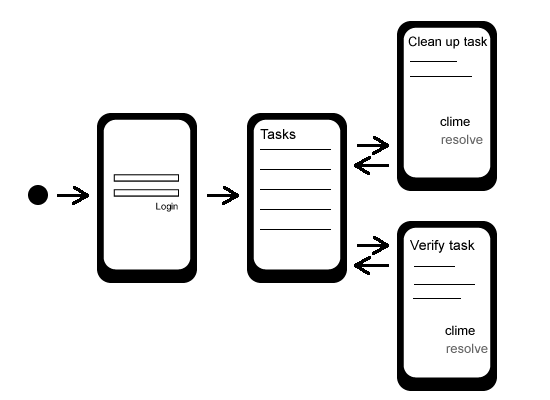
\includegraphics[scale=0.6]{activityFlowDiagram}}
\caption{Ekrany w aplikacji mobilnej wraz z przepływem komunikacji.}
\label{fig:activityFlowDiagram}
\end{figure}

Na rysunku~\ref{fig:activityFlowDiagram} przedstawiono przepływ komunikacji pomiędzy ekranami aplikacji. Po starcie domyślnie uruchamiany jest ekran logowania, który po poprawnym zalogowaniu otwiera główny ekran aplikacji czyli listę zadań. Z listy zadań w zależności od wybranego typu zadania użytkownik przenoszony jest do szczegółów, gdzie może wykonać akcję przypisania do zadania lub jego rozwiązania jeśli jest przypisany. 

\begin{figure}[h]
\centerline{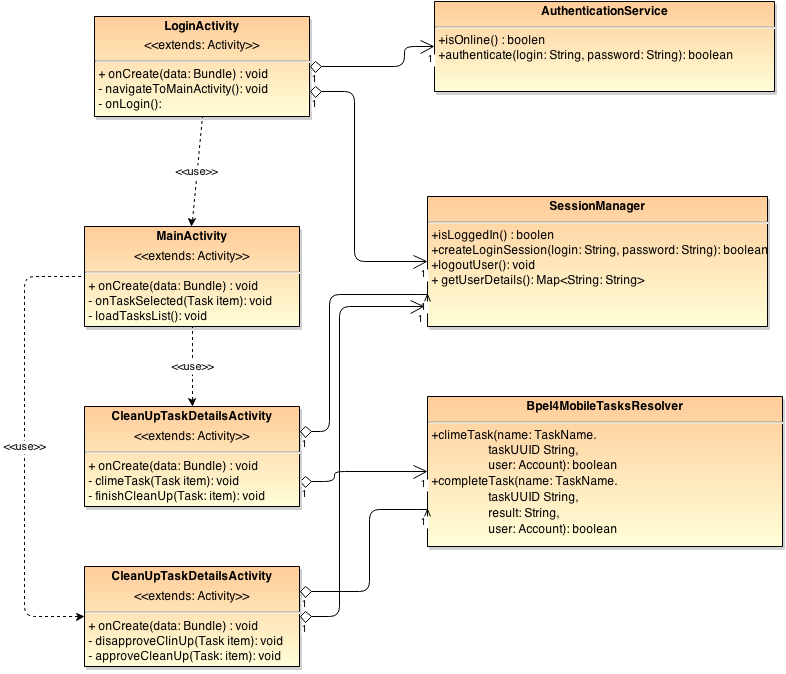
\includegraphics[scale=0.6]{activitiesClassDiagram}}
\caption{Diagram klas odpowiedzialnych za działanie poszczególnych ekranów.}
\label{fig:activitiesClassDiagram}
\end{figure}

Więcej szczegółów implementacyjnych poszczególnych ekranów widać na rysunku~\ref{fig:activitiesClassDiagram}, przedstawia on diagram klas poszczególnych ekranów oraz serwisów z których te klasy korzystają. Ekran logowania korzysta z serwisu do autoryzacji, który autoryzuje użytkownika wysyłając żądanie do warstwy pośredniej. Drugim z serwisów wykorzystywanych przez ekran logowania jest zarządca sesji, który odpowiada za utworzenie sesji użytkownika, w celu przechowywania jego danych dla pozostałych ekranów. Ekran główny wyszukuje listę zadań użytkownika bezpośredni z bazy danych, nie korzysta z innych serwisów. Ekrany szczegółów poszczególnych zadań wykorzystuje zarówno zarządcę sesji jak i serwis przeznaczony do komunikacji z warstwą pośrednią w celu przypisania lub rozwiązania zadania. 

W celu rozwiązania problemu synchronizacji listy zdań, skorzystano z interfejsów udostępnianych przez platformę android. Każda aplikacji przeznaczona na tą platformę posiada główny plik konfiguracyjny zwany \textit{AndroidManifest.xml}. W pliku tym zostały wskazane dwa serwisy implementujące interfejs serwisu udostępniony przez platformę, odpowiedzialne za udostępnienie adaptera do synchronizacji i~implementacje zarządcy kont użytkowników. 
\begin{figure}[h]
\centerline{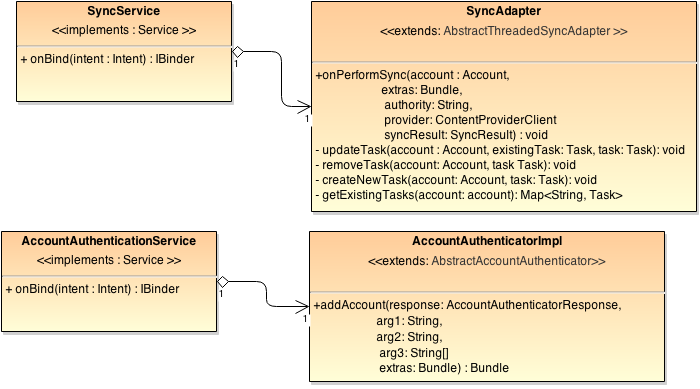
\includegraphics[scale=0.6]{androidSyncClasses}}
\caption{Diagram klas odpowiedzialnych za synchronizację.}
\label{fig:androidSyncClasses}
\end{figure}

Rysunek~\ref{fig:androidSyncClasses} przedstawia diagram wyżej wymienionych klas. Cykl życia adaptera synchronizacji, udostępnionego przez odpowiedni serwis, zarządzany jest przez system operacyjny. Proces synchronizacji uruchamiany jest cyklicznie na podstawie danych statystycznych o ilości zsynchronizowanych rekordów zwracanych przez adapter. Synchronizacja uruchamiana jest tylko w momencie dostępu aplikacji do Internetu, bez konieczności jej uruchamiania. Dzięki takiemu działaniu adaptera lista zadań aktualizowana jest mimo że użytkownik nie korzysta z aplikacji i jest zawsze aktualna kiedy użytkownika zechce z niej korzystać mimo braku dostępy do Internetu.

Implementacja zarządcy użytkownikami, jest konieczna do utworzenia kona użytkownika w systemie operacyjnym. Konto to jest wykorzystywane do synchronizacji. 

\subsection{Uruchomienie}

Aplikacja podobnie jak pozostałe systemy jest budowana przy pomocy narzędzia maven. Po poprawnym zbudowaniu aplikacji powstaje plik o rozszerzeniu apk, który może być bezpośrednio zainstalowany na urządzeniu mobilnym z systemem android.

